% Charlotte Geiger - Manuel Lippert - Leonard Schatt
% Physikalisches Praktikum

% Teilauswertung 1

\section{Qualitative Beobachtung verschiedener Kreiselbewegungen}

%\begin{itemize}
 %   \item Diskussion Beobachtung Stroboskop
  %  \item Bewegung Figurenachse im L-System und Drehimpulsachse bei Nutation
   % \item Entspricht Bewegungsrichtung ihren Erwartungen
    %\item Folge von $J_1 \approx J_3$
%\end{itemize}

Im Nachhinein wurde uns bewusst, dass wir einige Fehler bei der in der quantitativen Beobachtung gemacht haben. 
Dazu muss erstmal ein Fehler im Protokoll ausgebessert werden. Die Nutation ist nicht wie in Teil 1 fälschlicherweise 
behauptet, sondern gegen den Uhrzeigersinn, was später in der qualitativen Beobachtung auffiel. Nun zu den Beobachtungen.
\begin{itemize}
    \item Grundzustand:\\
        Der Kreisel wird nur angedreht. Alles verhält sich wie erwartet. Bei hohen Umdrehungszahlen ist eine kleine Nutation zu erkenne. Dies liegt vermutlich daran, dass der Kreisel
        leicht unsymetrisch ist. Der Effekt ist jedoch nur minimal und daher vernachlässigbar.
    \item Ohne Stroboskop:\\
        Nach dem Andrehen wurden auf den Kreisel mit den Fingern kräfte ausgeübt. Dabei war auffällig, dass je schneller der Kreisel sich dreht, desto stärker waren die Gegenkraft und Gefühlt war die Ausweichbewegung 
        stärker. Dies stimmt jedoch nicht mit den Fragen zur Vorbereitung und auch nicht mit der quantitativen Beobachtung überein. Diese Beobachtung kann daher kommen, 
        dass der kräftigere Gegendruck und die heftigere Reibung auf der Haut einem fälschlicherweise ein Gefühl des stärkeren Ausweichens geben.
        %Dabei war in der qualitativen Messung noch nicht klar ersichtlich, ob das stärkere Ausweichen 
        %von der höheren Drehfrequenz und dem damit verbundenen stärkeren "Abrollen" an dem Finger oder von der Präzession kommt.
        Die auftretende Ausweichgewegung war immer 
        senkrecht zu Rotationsachse und der Richtung in die die Kraft wirkt. \\
        Im Folgenden wurde das Gewicht an der Achse des Kreisel angebracht. Dabei konnte beobachtet werden, dass, wenn der Kreisel geneigt war und das Gewicht an ihm zieht, er auch wieder 
        eine Ausweichbewegung startet. In diesem Fall kann man sehr schön die Richtung der einwirkenden Kraft mit den Richtungen des Drehimpulses und der resultierenden Kraft beobachten.
        Diese lässt sich anhand der Drei-Finger-Regel herleiten.\\
        Die durch die Gravitation entstehende Kraft $F_{Grav}$ kann aufgespalten werden in einen Anteil $F_{\bot}$, der senkrecht zur Figurenachse ist, und einen der parallel Anteil $F_{\| }$. 
        Die Verhältnisser, in der sich die Gewichtskraft aufteilt, werden durch den Winkel der Drehachse und der Horizontalen. Wir haben zwei Ausrichtungen ausprobiert. Auffällig war, dass die 
        Kreisbewegung schneller zu sein schien, wenn die Drehachse parallel zu Horizont war als wenn der Kreisel in der $45\circ$-Position stand. DaFür die auf den 
        Kreisel wirkende Kraft $F_{\bot}$ gilt:
    \begin{equation*}
        F_{\bot} = F_{Grav} \cdot cos(\phi)
    \end{equation*}
    wobei $\phi$ der Winkel zwischen der Horizontalen und Drehachse ist.
    Daran ist klar zu erkennen, dass die Stärke der Präzision von der Größe der auf den Kreisel wirkenden Kraft abhängt.
    \item Mit Stroboskop:\\
        Die Nutation kann dadurch beobachtet werden, dass man das Stroboskop auf die Eigenfrquenz des Kreisels stellt. In der Praxis achtet man darauf, dass die Farbskala gleich bleibt. Nun betrachtet man, wie sich 
        die Stange mit der Zeit bewegt. Hier als Beispiel die beobachtete Nutation aus dem Versuch:\\
        \begin{figure}[h]
            \centering
            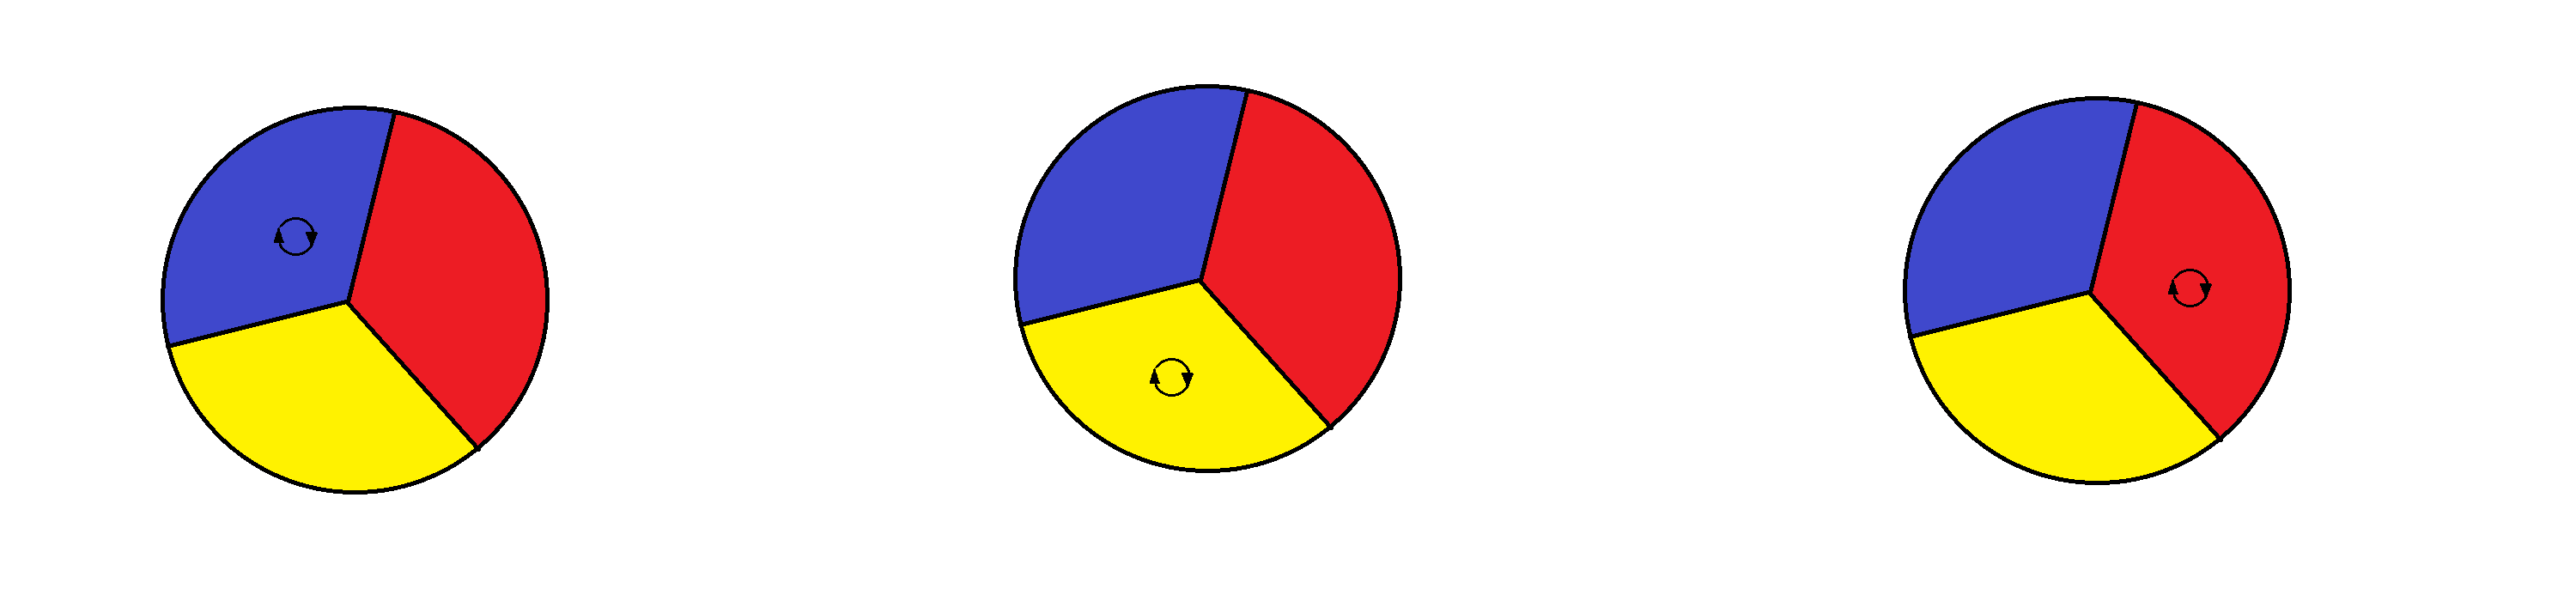
\includegraphics[width = 13cm]{Bilder/Leo/Nutationfarben.png}
            \caption{Schematische Darstellung der Kreisels von oben}
        \end{figure}
        Der Mittelpunkt des von der Strange beschreiben Kreis ist der Punkt durch den die Momentane Drehachse verläuft.
        Die Gangpolkegel rollt, wie in den Abbildung 4.2 oder in Kapitel 2.4
        dargelegt, außen an dem Raspolkegel ab, da $J_3 < J_1 = J_2$.
        \begin{figure}[h]
            \centering
            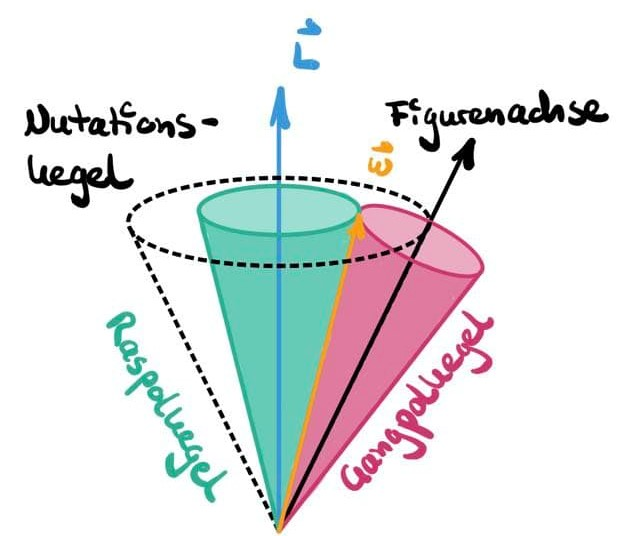
\includegraphics[scale = 0.3]{Bilder/6_1-Nutationsbewegung.jpg}
            \caption{Abrollen des Gangpolkegel außen am Raspolkegel}
        \end{figure}

\end{itemize}
\newpage